\section{Submodular}

\begin{frame}{Submodular}{Submodular}
	\begin{block}{}
		\begin{equation}
		\nonumber
		f(x_{1} , \cdots , x_{N} )= f(x_{1}) + \cdots + f(x_{N})
		\end{equation}
	\end{block}
\end{frame}

\begin{frame}{Sensor placement}{Maximum coverage}
\begin{figure}
	\centering
	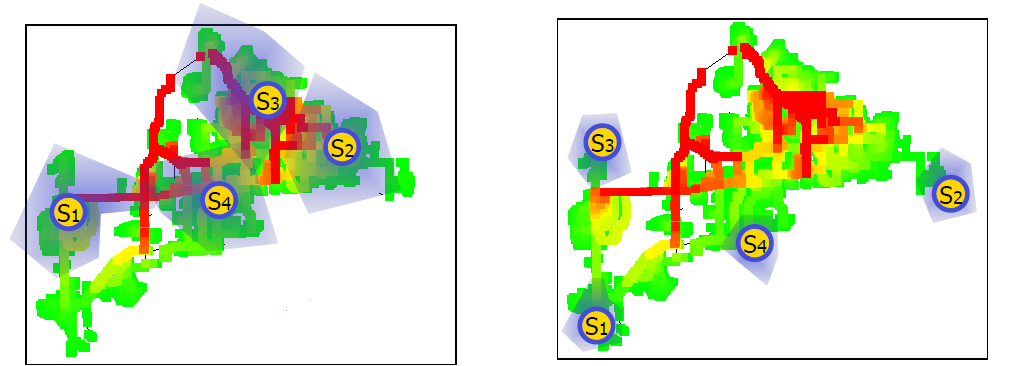
\includegraphics[width = \textwidth]{./figure/maximum_coverage}
\end{figure}	
\end{frame}

\begin{frame}{Sensor placement}{MAP inference}
\begin{figure}
	\centering
	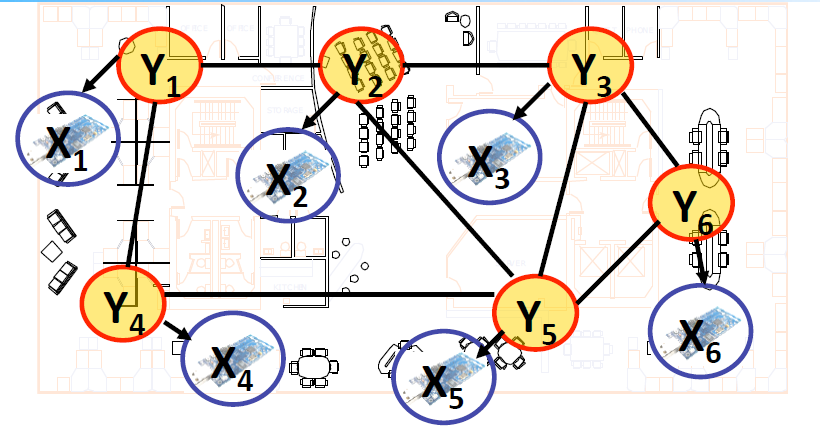
\includegraphics[width = \textwidth]{./figure/map_inference}
\end{figure}		
\end{frame}

\begin{frame}{Submodularity}{Definition}
\begin{block}{Definition}
Let $ N $ be a finite ground set and $ f : 2^{N} \rightarrow R $. Then $ f $ is \textbf{submodular} if $ \forall A, B \subseteq N,
f(A) + f(B) \leq f(A \cup B) + f(A \cap B). $
\end{block}
\begin{itemize}
\item diminishing returns
\item equivalence : $ f(x \cup S) \leq f(x) + f(S) $
\end{itemize}
\end{frame}

\begin{frame}{Submodular+Supmodular+Modular}{Relationship}
\begin{block}{Supmodular}
$ - f(x) $ is submodular $ \Rightarrow $ $ f(x) $ is supmodular.
\end{block}
\begin{block}{Modular}
$ f(x) $ is both submodular and supmodular, $ f(x) $ is modular.
\begin{equation}
\nonumber
f( \mathbf{X} ) = \sum_{ x_{i} \in \mathbf{X} } f(x_{i})
\end{equation}
\end{block}
\end{frame}

\begin{frame}{Submodular}{Performance guarantee}
\begin{block}{Theorem [Nemhauser et al `78]}
Suppose $ f $ is monotonic and submodular. 
Then greedy algorithm gives constant factor approximation.
\begin{equation}
\nonumber
f()
\end{equation}	
\end{block}
\begin{itemize}
\item Near-optimal
\item 
\end{itemize}
\end{frame}